\begin{frame}{Summarizing Data}
    Chapter 2 is all about summarizing data through summary statistics and graphs. We can get a lot of information out of these things!
    
    \vspace{12pt}
    These concepts are also important foundations for the rest of the course.
\end{frame}

\begin{frame}{Numerical Data}
    Let's start by thinking of a simple numeric variable: the ages of everyone in this room.
    
    \vspace{18pt}
    Can you think of any ways to summarize all of our ages in only one or two numbers?
\end{frame}

\begin{frame}{Scatterplots}
    A \textbf{scatterplot} shows a case-by-case view of two numerical variables. 
    
    \begin{center}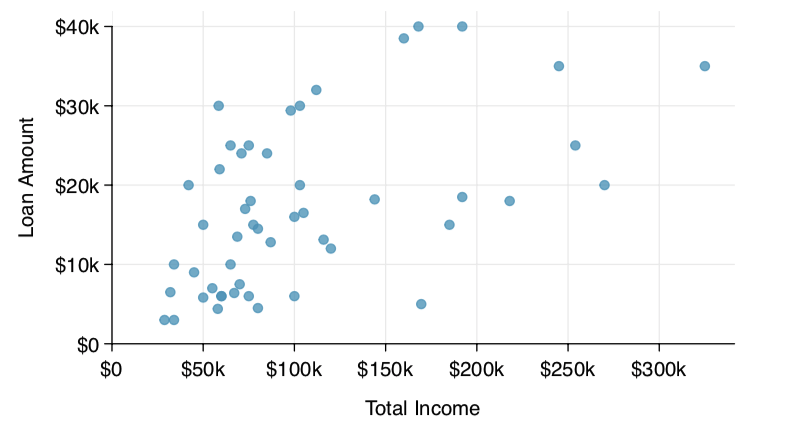
\includegraphics[scale=0.3]{images/scatter2.png}\end{center}
    
    What can we learn from the scatterplot?
\end{frame}

\begin{frame}{Dot Plots}
    A \textbf{dot plot} is like a scatterplot with only one variable. It shows how a single, \textit{continuous} numerical variable falls on a number line. 
    
    \begin{center}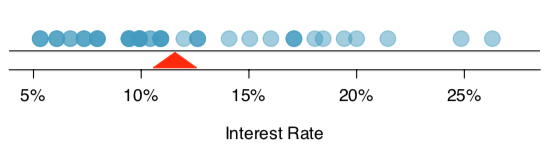
\includegraphics[scale=0.5]{images/dotplot.png}\end{center}
    
\end{frame}

\begin{frame}{Dot Plots}
    A \textbf{stacked dot plot} shows the same information for a \textit{discrete} numerical variable.   
    
    \begin{center}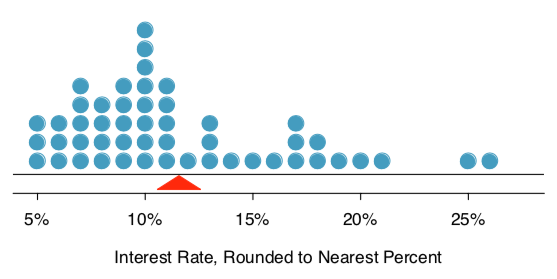
\includegraphics[scale=0.5]{images/dotplot2.png}\end{center}
\end{frame}

\begin{frame}{Histograms}
    A \textbf{histogram} is similar to a dot plot, but instead of showing the exact value for each observation, values are put into \textbf{bins}.
    
    \begin{center}
        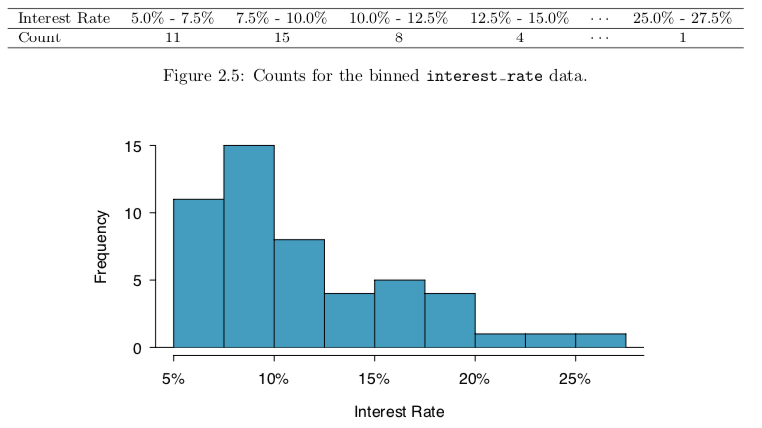
\includegraphics[scale=0.4]{images/hist1.png}
    \end{center}
\end{frame}

\begin{frame}{The Mean}
    Both of the dot plots had a red arrow pointing to the \textbf{mean} (or \textbf{average}) of the variable. 
    
    \vspace{12pt}
    You've probably calculated an average before, but if you haven't (or if you need a refresher), to find the mean you add all of the values and then divide by the number of values. 
\end{frame}

\begin{frame}{The Mean}
    For example, if we had a variable called \texttt{ages} with the values 21, 22, 26, 18, 19, and 21, the mean would be
    \vspace{12pt}
    \[
    \frac{\text{sum of values}}{\text{total \# of observations}} = \frac{21+22+26+18+19+21}{6}.
    \]
    
    \vspace{12pt}
    We denote the mean by $\boldsymbol{\bar{x}}$. In this case, $\bar{x}=21.167$
\end{frame}

\begin{frame}{The Mean}
    In math notation, the formula for the mean looks like this:
    \[
        \bar{x} = \frac{1}{n}\sum_{i=1}^n x_i = \frac{x_1 + x_2 + \dots + x_n}{n}.
    \]
    
    \vspace{12pt}
    In our example, $n=6$ observations and each $x_i$ is one of our ages.
\end{frame}

\begin{frame}{Measures of Center}
    The mean is a common way to measure the center (middle) of the \textbf{distribution} of the data.
    
    \vspace{12 pt}
    You can think of the distribution as the way that the data is \textit{distributed} from left to right on a histogram.
\end{frame}

\begin{frame}{Measures of Center}
    The mean of a variable is denoted by $\bar{x}$. This is what we refer to as the \textbf{sample mean}. 
    
    \vspace{12pt}
    The mean of the entire population is typically something that we don't have exact data on (we usually don't have data for every single member of a population). Instead, we estimate the population mean using a sample mean.
    
    \vspace{12pt}
    The \textbf{population mean} is denoted by $\boldsymbol{\mu}$. This is the Greek letter \textit{mu}.
\end{frame}

\begin{frame}{That's a lot of symbols to remember?}
    Let's put them all in one place. We will add to this list as we go.
    \begin{itemize}
        \item $n$: number of observations/cases
        \item $\bar{x}$: sample mean
        \item $\mu$: population mean
    \end{itemize}
\end{frame}

\begin{frame}{Data Density}
    Now that we've brought up the distribution of the data, we can start to think about the density of the data.
    
    \vspace{12pt}\textbf{Data density} refers to the amount of data in any bin. (Taller bins mean more data density, or more data in the bin.)
    
    \vspace{12pt}From here, we can start to consider the \textit{shape} of a distribution. 
\end{frame}

\begin{frame}{Shape}
    Remember our histogram?
    
    \begin{center}
        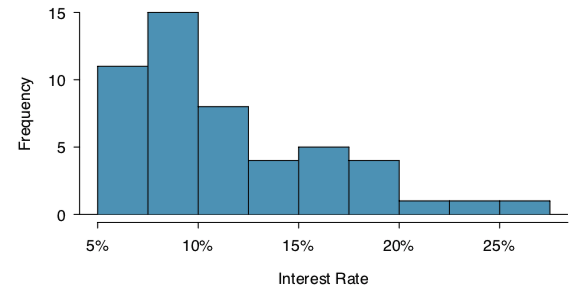
\includegraphics[scale=0.3]{images/hist2.png}
    \end{center}
    
    \begin{itemize}
        \item The sides of the distribution (on either side of the mean) are referred to as the \textbf{tails}. 
        \item Here the data have a long, thin right tail, so we say that the shape is \textbf{right skewed}. 
    \end{itemize}
\end{frame}

\begin{frame}{Shape}
    \begin{itemize}
        \item If the data have a long, thin tail on the left, we say that the shape is \textbf{left skewed}.
        \item If the data have roughly equal tails, we say the distribution is \textbf{symmetric}. 
    \end{itemize}
\end{frame}

\begin{frame}{Shape}
    We can also talk about the modes of a distribution. In a distribution, a \textbf{mode} is any prominent peak in the distribution. These can be found in a histogram! 
    \begin{itemize}
        \item A distribution with one prominent peak is called \textbf{unimodal}.
        \item Distributions with two prominent peaks are \textbf{bimodal}.
        \item Distributions with three or more promiment peaks are \textbf{multimodal}. 
    \end{itemize}
\end{frame}

\begin{frame}{Modes}
    \begin{center}
        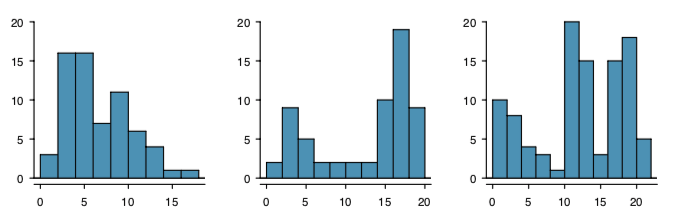
\includegraphics[scale=0.5]{images/modes.png}
    \end{center}
    
    How many modes are there in each distribution? \\ Remember that we only count \textit{prominent} peaks.
\end{frame}

\begin{frame}{Modes}
    Bin widths, our particular sample, and differing opinions can all impact where we see a "prominent" mode.
    
    \vspace{12pt} ...but that is okay! The goal of examining the shape of our data is simply to better understand the nature of our data. This allows us to make more informed technical decisions down the line. 
\end{frame}

\begin{frame}{Variability}
    We talked about the mean as a way to measure the center of the data, but the variability of data is also an important consideration. 
    
    \vspace{12pt}
    Why might the variability be important?
\end{frame}

\begin{frame}{Why Variability?}
    Suppose we want to know the average age in this class and take two random samples of size 10 each. 
    
    \begin{table}[]
    \begin{tabular}{ll}
    Sample 1: & 22, 19, 20, 18, 20, 21, 20, 22, 20, 18\\ 
    \hline
    Sample 2: & 12, 18, 32, 21, 19, 19, 17, 21, 22, 19
    \end{tabular}
    \end{table}

    In both cases, we get a sample average of $\bar{x}=20$.
    
    \vspace{12pt}How confident are you about our estimate of the average age in this class using Sample 1? What about Sample 2?
\end{frame}

\begin{frame}{Variability}
    We can think about variability as how far away the observations are from the mean. 
    
    \vspace{12pt}The distance between an observation and its mean is called the \textbf{deviation}. From Sample 1 (22, 19, 20, 18, 20, 21, 20, 22, 20, 18), the deviations for the first, second, and tenth observations are
    \begin{align*}
        x_1 - \bar{x} &= 22-20 = 2 \\
        x_2 - \bar{x} &= 19-20 = -1 \\
        x_{10}-\bar{x} &= 18-20=-2
    \end{align*}
\end{frame}

\begin{frame}{Variability}
    We're interested in how far a typical observation is from the mean, but if we add up all of the deviations for a sample, we always get zero! Let's try it on Sample 1:
    
    \begin{align*}
        & (x_1 - \bar{x}) + (x_2 - \bar{x}) + \dots + (x_9 - \bar{x}) + (x_{10} - \bar{x}) \\
        &= (22-20) + (19-20) + (20-20) + (18-20) + (20-20) \\ & \quad + (21-20) + (20-20) + (22-20) + (20-20) + (18-20) \\
        &= 2 + (-1) + 0 + (-2) + 0 + 1 + 0 + 2 + 0 + (-2) \\
        &= 2 - 1 - 2 + 1 + 2 - 2 \\
        &= 0
    \end{align*}
    
    Note: A short proof of this will be posted on the course website.
\end{frame}

\begin{frame}{Variability}
    So the average deviance doesn't work... 
    \begin{itemize}
        \item This is because all of those positives and negatives end up balancing each other out. 
        \item When we talk about variability, we aren't that interested in whether any particular point is above or below the mean.
        \item We really just want to know how far away it is.
    \end{itemize}
\end{frame}

\begin{frame}{Variability}
    There are two simple ways to get rid of the signs to focus on distance (without direction).
    \begin{enumerate}
        \item Take the absolute value of the number.
        \item Square the number.
    \end{enumerate}
    
    \vspace{12pt}It turns out that there are a whole lot of mathematical reasons why it's easier to work with squares than with absolute values!
\end{frame}

\begin{frame}{Variance}
    And so we come to the \textbf{variance}. The variance can be inconvenient to calculate by hand, but it goes something like this:
    \begin{enumerate}
        \item We square all of those deviations we calculated previously.
        \item Add them up.
        \item Take the average.
    \end{enumerate}
    We denote our \textbf{sample variance} by $\boldsymbol{s^2}$.
\end{frame}

\begin{frame}{Variance}    
    \vspace{12pt}Note: Technically, we divide by $n-1$ instead of by $n$ when we take our average. We may talk more about this later, but in the meantime just know that there's some mathematical nuance that makes the variance formula a little bit more complicated. 
\end{frame}

\begin{frame}{Variance}
    Let's return to our example and Sample 1. We already calculated our deviations, but this time we square them before adding them up.
    \begin{align*}
        & (22-20)^2 + (19-20)^2 + \dots + (20-20)^2 + (18-20)^2 \\
        & = 2^2 + (-1)^2 + 0^2 + (-2)^2 + 0^2 + 1^2 + 0^2 + 2^2 + 0^2 + (-2)^2 \\
        &= 4 + 1 + 4 + 1 + 4 + 4 \\
        &= 18
    \end{align*}
    And then we divide by $n-1=9$
    \[
    \frac{18}{9}=2.
    \]
\end{frame}

\begin{frame}{Standard Deviation}
    The variance can be described as the average squared distance from the mean. That probably doesn't sound like a very intuitive way to measure variability.
    
    \vspace{12pt}However, the \textbf{standard deviation} is easier to conceptualize than the variance: it gets at our original goal of estimating how far a typical observation is from the mean.
\end{frame}

\begin{frame}{Standard Deviation}
    Fortunately for us, the standard deviation doesn't require any additional mathematical nuance! In order to calculate the standard deviation, we simply take the square root of the variance.
    
    \vspace{12pt}Returning again to our example, 
    \[
    s = \sqrt{s^2} = \sqrt{2} \approx 1.414
    \]
\end{frame}

\begin{frame}{Standard Deviation}
    In general,
    \begin{itemize}
        \item 70\% of the data will fall within one standard deviation of the mean.
        \item 95\% of the data will fall within two standard deviations of the mean.
    \end{itemize}
    ...but these are not strict rules!
\end{frame}

\begin{frame}{Population Variability}
    Like the mean, the \textbf{sample variance} and \textbf{sample standard deviation} also have population counterparts.
    \begin{itemize}
        \item The \textbf{population variance} is denoted $\boldsymbol{\sigma^2}$.
        \item The \textbf{population standard deviation} is denoted $\boldsymbol{\sigma}$.
    \end{itemize}
    $\sigma$ is the Greek letter \textit{sigma}. (We often use Greek letters to denote values from our population.)
\end{frame}

\begin{frame}{Mean and Standard Deviation}
    Much of what we do in statistics is (1) estimate quantities and (2) determine how uncertain we are about those estimates. 
    \begin{itemize}
        \item The mean is often a quantity of interest.
        \item The standard deviation helps us determine how uncertain we are about this quantity.
    \end{itemize}
    
    \vspace{12pt}We will talk more about uncertainty in Chapter 5.
\end{frame}

\begin{frame}{Symbols to Remember}
    Let's update our list with variance and standard deviation.
    \begin{itemize}
        \item $n$: number of observations/cases
        \item $\bar{x}$: sample mean
        \item $\mu$: population mean
        \item $s^2$: sample variance
        \item $s$: sample standard deviation
        \item $\sigma^2$: population variance
        \item $\sigma$: population standard deviation
    \end{itemize}
\end{frame}

\begin{frame}{Mean, Standard Deviation, and Shape}
    Mean, standard deviation, and shape together give us a good description of our distribution. 
    \begin{itemize}
        \item If any one of these is missing, we miss crucial information.
        \item Without the mean, we lack information about the center of the distribution.
        \item Without the standard deviation, we are unable to capture how spread out the data are. 
    \end{itemize}
\end{frame}

\begin{frame}{Why Shape?}
    These three distributions have the same mean ($\bar{x}=0$) and standard deviation ($s=1$)!
    \begin{center}
        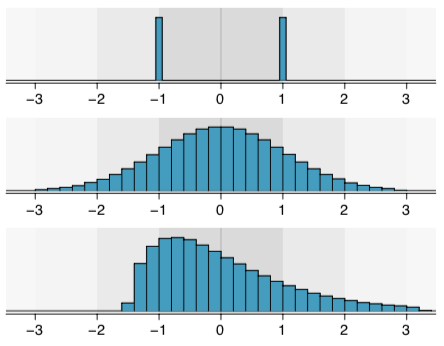
\includegraphics[scale=0.35]{images/shapes.png}
    \end{center}
    A good description of shape should include modality and skewness (or symmetry). To give an even clearer picture, we can report where the modes are and the sharpness of the peaks.
\end{frame}

\begin{frame}{Box Plots}
    \begin{center}
        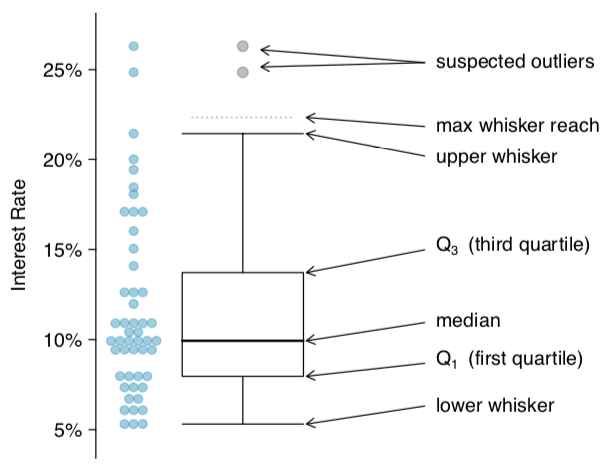
\includegraphics[scale=0.4]{images/boxplot.png}
    \end{center}
    A stacked dot plot next to a vertical box plot. 
\end{frame}

\begin{frame}{The Median}
    The first step in constructing a box plot is to draw a line at the median. 
    
    \begin{center}
        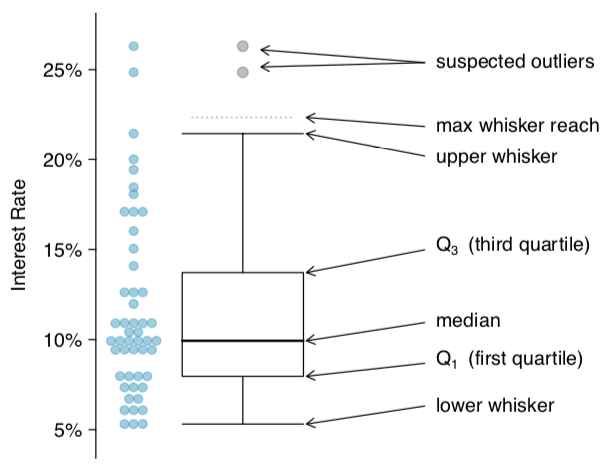
\includegraphics[scale=0.35]{images/boxplot.png}
    \end{center}
\end{frame}

\begin{frame}{The Median}
    \begin{itemize}
        \item The \textbf{median} takes the data and splits it in half. 
        \item The median is also called the \textbf{50th percentile} because 50\% of the data is below this value.
        \item The median is another measure of center. 
        \item To find the median, we sort our numerical variable and then find the halfway point.
    \end{itemize}
\end{frame}

\begin{frame}{The Median}
    If we have an odd number of observations, say,
    \[
        1,2,3,4,5
    \]
    we take the observation in the middle (the $\frac{n+1}{2}$th observation).
   
   \vspace{12pt}In this case,
    \[
        1,2,\boldsymbol{3}, 4, 5
    \]
    3 is the median. 
\end{frame}

\begin{frame}{The Median}
    \begin{itemize}
        \item If we have an even number of observations
        \[
        1,2,3,4,5,6
        \]
        we cut the data exactly in half
        \[
        1,2,3 \quad|\quad 4,5,6
        \]
        and the median is the average of the two observations closest to the halfway point
        \[
        \frac{3+4}{2}=3.5
        \]
    \end{itemize}
\end{frame}

\begin{frame}{Quartiles}
    The next step in our box plot is to draw a box connecting the first and third quartiles.
    
    \begin{center}
        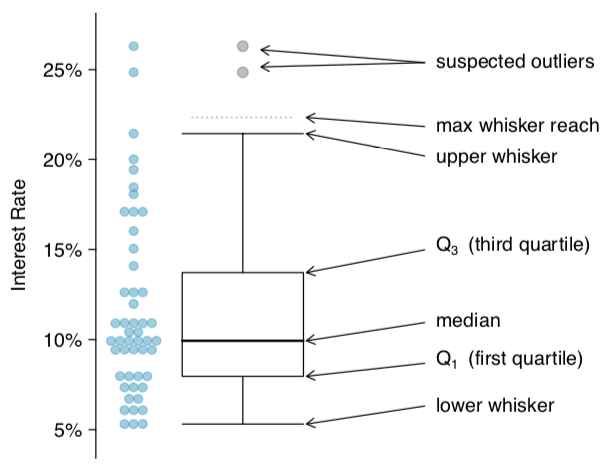
\includegraphics[scale=0.35]{images/boxplot.png}
    \end{center}
\end{frame}

\begin{frame}{Quartiles}
    \textbf{Quartiles} split our data into \textit{quarters}.
    \begin{itemize}
        \item 25\% of the data falls below the \textbf{first quartile} (Q1). 
        \begin{itemize}
            \item This is the 25th percentile. 
        \end{itemize}
        \item 50\% of the data falls below the median.
        \item 75\% of the data falls below the \textbf{third quartile} (Q3). 
        \begin{itemize}
            \item This is the 75th percentile. 
        \end{itemize}
    \end{itemize}
    
    \vspace{12pt}What percent of the data falls between Q1 and the median? What percent between Q1 and Q3?
\end{frame}

\begin{frame}{Finding Quartiles}
    \begin{enumerate}
        \item Find the median.
        \item Take all of the data that falls \textit{below} the median and find the middle of that data using the same steps we used to find the median. This is the first quartile.
        \item Repeat with the data that falls \textit{above} the median. This is the third quartile.
    \end{enumerate}
\end{frame}

\begin{frame}{Interquartile Range}
    \begin{itemize}
        \item The distance between the first and third quartiles is referred to as the \textbf{interquartile range} (or IQR).
        \item This value is easy to calculate!
        \[
        IQR = Q3 - Q1
        \]
        \item The IQR is another measure of variability.
    \end{itemize}
\end{frame}

\begin{frame}{Whiskers}
    Now we need to find the whiskers.
    \begin{center}
        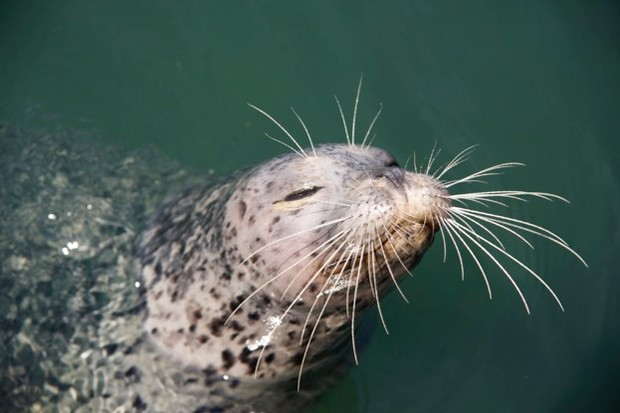
\includegraphics[scale=0.4]{images/whiskers.jpg}
    \end{center}
    \flushright\tiny{Image from BBC Wildlife \\ www.discoverwildlife.com/animal-facts/mammals/how-do-whiskers-work/}
\end{frame}

\begin{frame}{Whiskers}
    Now we need to find the whiskers.
    \begin{center}
        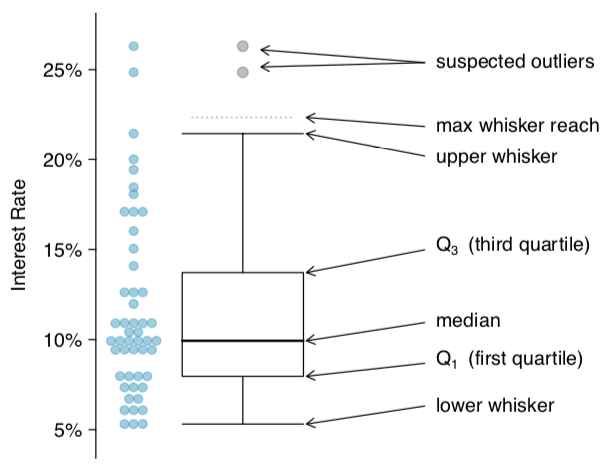
\includegraphics[scale=0.35]{images/boxplot.png}
    \end{center}
\end{frame}

\begin{frame}{Whiskers}
    The \textbf{whiskers} capture (most of) the rest of the data.
    \begin{itemize}
        \item Each whisker is no longer than 
        \[
        1.5\times IQR.
        \]
        and stops at the point closest to, but still within, this range.
    \end{itemize}
\end{frame}

\begin{frame}{Whiskers}
    \begin{itemize}
        \item The upper whisker goes no farther than
        \[
        Q3 + 1.5 \times IQR
        \]
        and the lower whisker no farther than
        \[
        Q1 - 1.5 \times IQR
        \]
    \end{itemize}
    
    We may choose not to include the maximum upper reach and minimum lower reach on our box plot, but we always include the whiskers themselves. 
\end{frame}

\begin{frame}{Outliers}
    Finally, we add any outliers by labeling each one with a dot.
    \begin{center}
        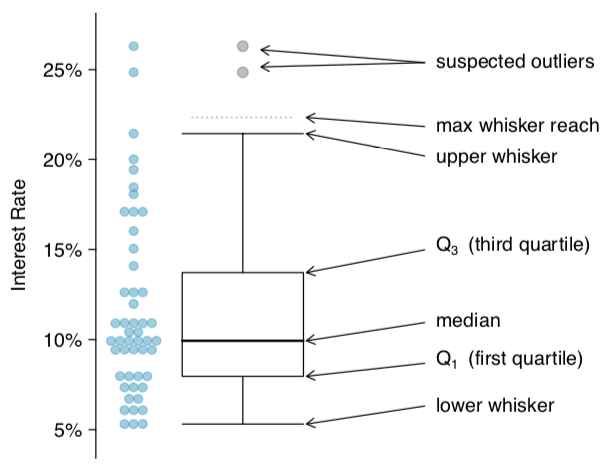
\includegraphics[scale=0.35]{images/boxplot.png}
    \end{center}
\end{frame}

\begin{frame}{Outliers}
    Since we've already built the rest of our boxplot, we can start to think about outliers as whatever is left out. 
    \begin{itemize}
        \item We label these observations specifically because they are \textit{unusual} or \textit{extreme}.
        \item Observations that are unusually far from the rest of the data are referred to as \textbf{outliers}.
    \end{itemize}
\end{frame}

\begin{frame}{Why Examine Outliers?}
    \begin{itemize}
        \item Identify sources of strong skew.
        \item Provide insight into potentially interesting properties of the data.
        \item Identify possible data collection or data entry errors.
    \end{itemize}
\end{frame}

\begin{frame}{Robust Statistics}
    Suppose we have some data:
    \[
    3,  6,  7,  4, 10,  8,  1,  5,  2,  9
    \]
    and I replace the largest observation (10) with a significantly larger value (35).
    \[
    3,  6,  7,  4, 35,  8,  1,  5,  2,  9
    \]
\end{frame}

\begin{frame}{Robust Statistics}
    For our original data,
    \[
    3,  6,  7,  4, 10,  8,  1,  5,  2,  9
    \]
    we get the following:
    \begin{table}[]
        \begin{tabular}{ccccc}
        median & $IQR$ & & $\bar{x}$ & $s$ \\ 
        \hline
        5.5 & 4.5 & & 5.5 & 3.03 
        \end{tabular}
    \end{table}
    
    \vspace{12pt}What do you think will happen to our sample statistics (mean, median, standard deviation, and IQR) when I replace 10 with 35?
\end{frame}

\begin{frame}{Robust Statistics}
    Replacing 10 with 35, these numbers shift somewhat:
    \begin{table}[]
        \begin{tabular}{lccccc}
        & median & $IQR$ & & $\bar{x}$ & $s$ \\ 
        \hline
        Original Data & 5.5 & 4.5 & & 5.5 & 3.03 \\
        Modified Data & 5.5 & 4.5 & & 8.0 & 9.83
        \end{tabular}
    \end{table}
    
    \vspace{12pt}The median and IQR are exactly the same, but the mean and standard deviation change quite a bit!
\end{frame}

\begin{frame}{Robust Statistics}
    We say that the median and IQR are \textbf{robust statistics} or that they are \textit{robust to} outliers, meaning that their values are minimally effected by these extreme observations. 
    \begin{table}[]
        \begin{tabular}{lccccc}
        & \multicolumn{2}{c}{Robust} && \multicolumn{2}{c}{Not Robust} \\
        \hline
        & median & $IQR$ & & $\bar{x}$ & $s$ \\ 
        \hline
        Original Data & 5.5 & 4.5 & & 5.5 & 3.03 \\
        Modified Data & 5.5 & 4.5 & & 8.0 & 9.83
        \end{tabular}
    \end{table}
    
    \vspace{12pt}Why do you think the mean and standard deviation changed so much, but the median and IQR did not?
\end{frame}

\begin{frame}{When Are Robust Statistics Important?}
    \begin{itemize}
        \item Suppose you wanted to know about the typical home price in the United States in 2018.
        \item Recall that the mean and median are both measures of center.
        \item Would you look at the mean or the median? Why?
    \end{itemize}
\end{frame}

\begin{frame}{When Are Robust Statistics Important?}
    As long as you can defend your answer, there is value to each option!
    \begin{itemize}
        \item If we wanted to know what the typical homeowner is spending, the median would be more useful.
        \item If we wanted our estimate to scale, e.g., to estimate how much total money was spent on homes in 2018, the mean might be a better option. 
    \end{itemize}
\end{frame}

\begin{frame}{Transforming Data}
    \begin{itemize}
        \item When data are very strongly skewed, we sometimes transform them to make them easier to model.
        \item For our purposes, data is easiest to model when it is 
        \begin{itemize}
            \item Mostly symmetric
            \item Unimodal
            \item "Bell-shaped"
        \end{itemize}
        \item We want to be able to use our mean and standard deviation instead of our median and IQR!
    \end{itemize}
\end{frame}

\begin{frame}{Transforming Data}
    What does it mean to "transform" the data?
    \begin{itemize}
        \item Essentially, we apply some mathematical function to our data in order to rescale it.
        \item Technically, we want transformations that are continuous and invertible.
        \item Fortunately, there are a number of standard transformations that we use. 
    \end{itemize}
\end{frame}

\begin{frame}{Example: Transforming Data}
    A histogram of the populations of all US counties.
    \begin{center}
        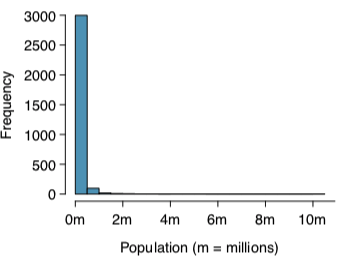
\includegraphics[scale=0.5]{images/trans1.png}
    \end{center}
    For perspective, Riverside County has 2.4 million people and \\ Los Angeles County has 10.2 million people!
\end{frame}

\begin{frame}{Example: Transforming Data}
    \begin{center}
        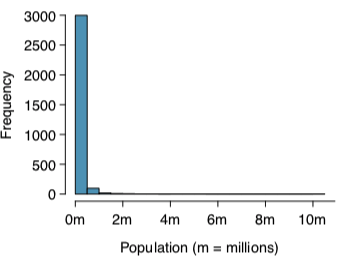
\includegraphics[scale=0.5]{images/trans1.png}
    \end{center}
    
    These data are very strongly skewed! Almost all of the counties have populations between 0 and 1 million people, but a few have over 10 million.
\end{frame}

\begin{frame}{Example: Transforming Data}
    To transform the data we take $\log_{10}(Population)$. The histogram of the transformed data looks like this:
    \begin{center}
        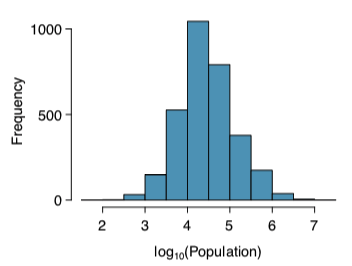
\includegraphics[scale=0.5]{images/trans2.png}
    \end{center}
\end{frame}

\begin{frame}{Example: Transforming Data}
    Before and after transformation:
    \begin{center}
        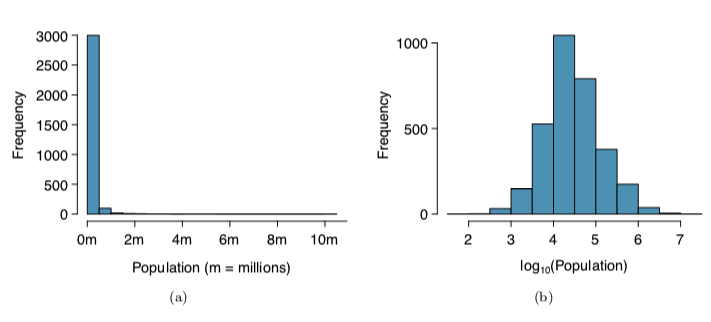
\includegraphics[scale=0.45]{images/transform.png}
    \end{center}
    In histogram (b), it is much more reasonable to use the mean and standard deviation to measure the center and spread of our data.
\end{frame}

\begin{frame}{Transformations}
    We may also apply
    \begin{itemize}
        \item A square root transformation
        \begin{itemize}
            \item $\sqrt{\text{original variable}}$
        \end{itemize}
        \item An inverse transformation
        \begin{itemize}
            \item $(\text{original variable})^{-1}$
        \end{itemize}
    \end{itemize}
\end{frame}

\begin{frame}{Transformations}
    In general, transformations:
    \begin{itemize}
        \item Let us see data structure differently.
        \item Reduce skew.
        \item Assist in modeling.
        \item Straighten nonlinear relationships in scatterplots.
    \end{itemize}
\end{frame}

\begin{frame}{Visualizing Geographic Data}
    \begin{itemize}
        \item Geographic data can be plotted using the data visualization techniques we've already seen.
        \item We might instead want to create an intensity plot.
        \item These plots allow us to show higher and lower values of a variable using colors on a map.
        \item Intensity plots are good for seeing geographic trends.
    \end{itemize}
\end{frame}

\begin{frame}{Mapping Data}
    \begin{center}
        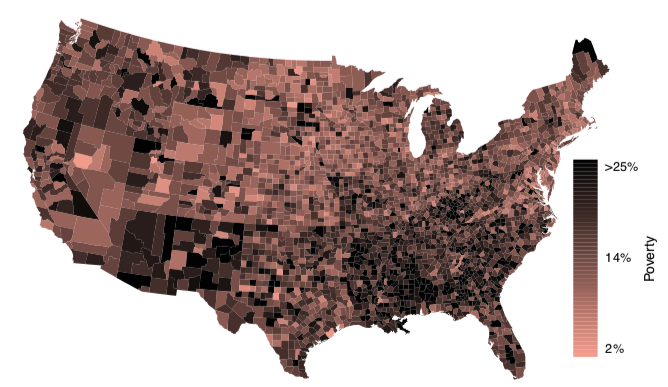
\includegraphics[scale=0.5]{images/map.png}
    \end{center}
\end{frame}

